%% grundlagen.tex
%% $Id: grundlagen.tex 28 2007-01-18 16:31:32Z bless $
%%

\chapter{Basics \& Related Work}
\label{ch:Basics}

\section{Schlafmedizin}
\label{ch:Basics:se:schlafmedizin}
% start seite 3-5 im buch schlafmedizin_1x1 
Unter dem Begriff \textit{Schlafmedizin} versteht man die Lehre von Diagnostik, Klassifikation und Behandlung von Störungen währrend des Schlafs \cite{schlafmedizin_1x1}. 
Trotz Erwähnungen in der Antike findet Schlafmedizin erst seit des letzten Jahrhunderts Bedeutung.
Mithilfe der Polysomnographie konnten unterschiedliche Schlafphasen zyklischen Ablaufs erkannt werden.
Zudem konnten den Schlafphasen physiologische Eigenschaften nachgewiesen werden.
Die Polysomnographie misst Gehirnströme, Augenbewegungen und Muskelspannungen.
Mithilfe dieser Informationen konnte man Schlafkrankheiten erkennen und mit der Behandlung dieser beginnen.


Heutzutage sind ca. 80 Schlafstörungen in dieversen Bereichen bekannt, welche neben psychologischen Testverfahren überwiegend elektrophysiologisch untersucht und behandelt werden.
Patienten werden mit ambulanten Hilfsmitteln oder stationär in einem Schlaflabor untersucht und anschließend von einem technisch ausgebildeten Personal analysiert.
Im Falle eines Schlaflabors, welches genauere Messergebnisse im Vergleich zu einem ambulanten Hilfsmittel (z.B eine Langzeitbewegungsmessung) liefert, wird eine Polysomnographie durchgeführt.
% ende cite
% start seite 9- im buch schlafmedizin_1x1 
Im Schlaflabor werden neben elektrophysiologischen Messungen des Schlafs auch Untersuchungen der Müdigkeit, der Tagesschläfrigkeit und der Aufmerksamkeit vorgenommen \cite{schlafmedizin_1x1}.
% ende cite

\todo{Seite 13,14 in 1x1, schlaf erklärt, wie psg was klassifiziert usw... wichtig!!!}

\section{Schlaf: Respiratorische Ereignisse}

\todo{Seite 81+ 1x1... anschauen, erklären, was respiratorische Ereignisse sind}

Welche respiratorischen Ereignisse gibt es \& wie unterscheiden sie sich (Apnoe, Hypopnoe, Hyperventilation, ...)?
\todo{Apnoes unterscheiden und erklären}

\subsection{Zentrales Schlafapnoe}
\todo{Zentrales apnoe im 1x1 auf 86 erklärt...}
\todo{Schlaf von Apnoepatienten 91 1x1}
\todo{126-127 in praxis der schlaf...}

\todo{Diagnostik 95 1x1}

\section{Klassifizierung von Schlafstörungen}
Schlafstörungen können durch die Möglichkeit, viele Biosignale währrend des Schlafes zu registrieren, genauer charaktisiert werden \cite{praxis_der_schlafmedizin}.
Basierend auf dieser Annahme wurden folgende Klassifikationen für Schlafstörungen entwickelt.
\begin{itemize}
    \item Ein- und Durchschlafstörungen (Insomnien)
    \item Schlafbezogene Atmungsstörungen
    \item Hypersomnien zentralnervösen Ursprungs
    \item Zirkadiane Rhythmusschlafwachstörungen
    \item Störungen in Verbindung mit Schlaf, Schlafstadien oder partiellem Erwachen (Parasomnien)
    \item Schlafbezogene Bewegungsstörungen
    \item Andere Schlafstörungen
\end{itemize}

Diese Gliederung orientiert sich an der \textit{ICSD-3} \cite{praxis_der_schlafmedizin}.

\todo{Welche Alternativen gibt es zur Aufzeichnung und Klassifikation?}

\section{Forschung von Klassifikation anhand von IMU-Daten}
Es gibt bereits Ansätze, welche sich damit befassen, Alternativen zur Ermittlung von Schlafstörungen zu finden. 
Somit könnte ein Besuch im Schlaflabor ersetzt werden durch einen bequemen Test.
Ein Ansatz ist es, mittels IMU-Daten die Bewegung des Körpers zu messen und anhand dieser Informationen die Atmung oder ähnliches herauszufiltern, um dann Rückschlüsse auf Schlafstörungen schließen zu können.

\subsection{Accelerometer am Brustkorb}

Bereits 2018 gab es Forschung in diesem Bereich, womit sich \textit{Phan Duy Hung} damit befasst hat, einen Accelerometer an den Brustkorb zu fixieren \cite{hung_central_2018}.
Es wurde versucht, durch die Platzierung an geanu dieser Stelle das Herzschlagen genauer erkennen zu können. 
Die Rohdaten zeigen hierbei bereits die Herzfrequenz und die Atmung des Probanden (siehe Abb. \ref{imu_research_hung_rawData}).

\begin{figure}[ht]
    \centering
    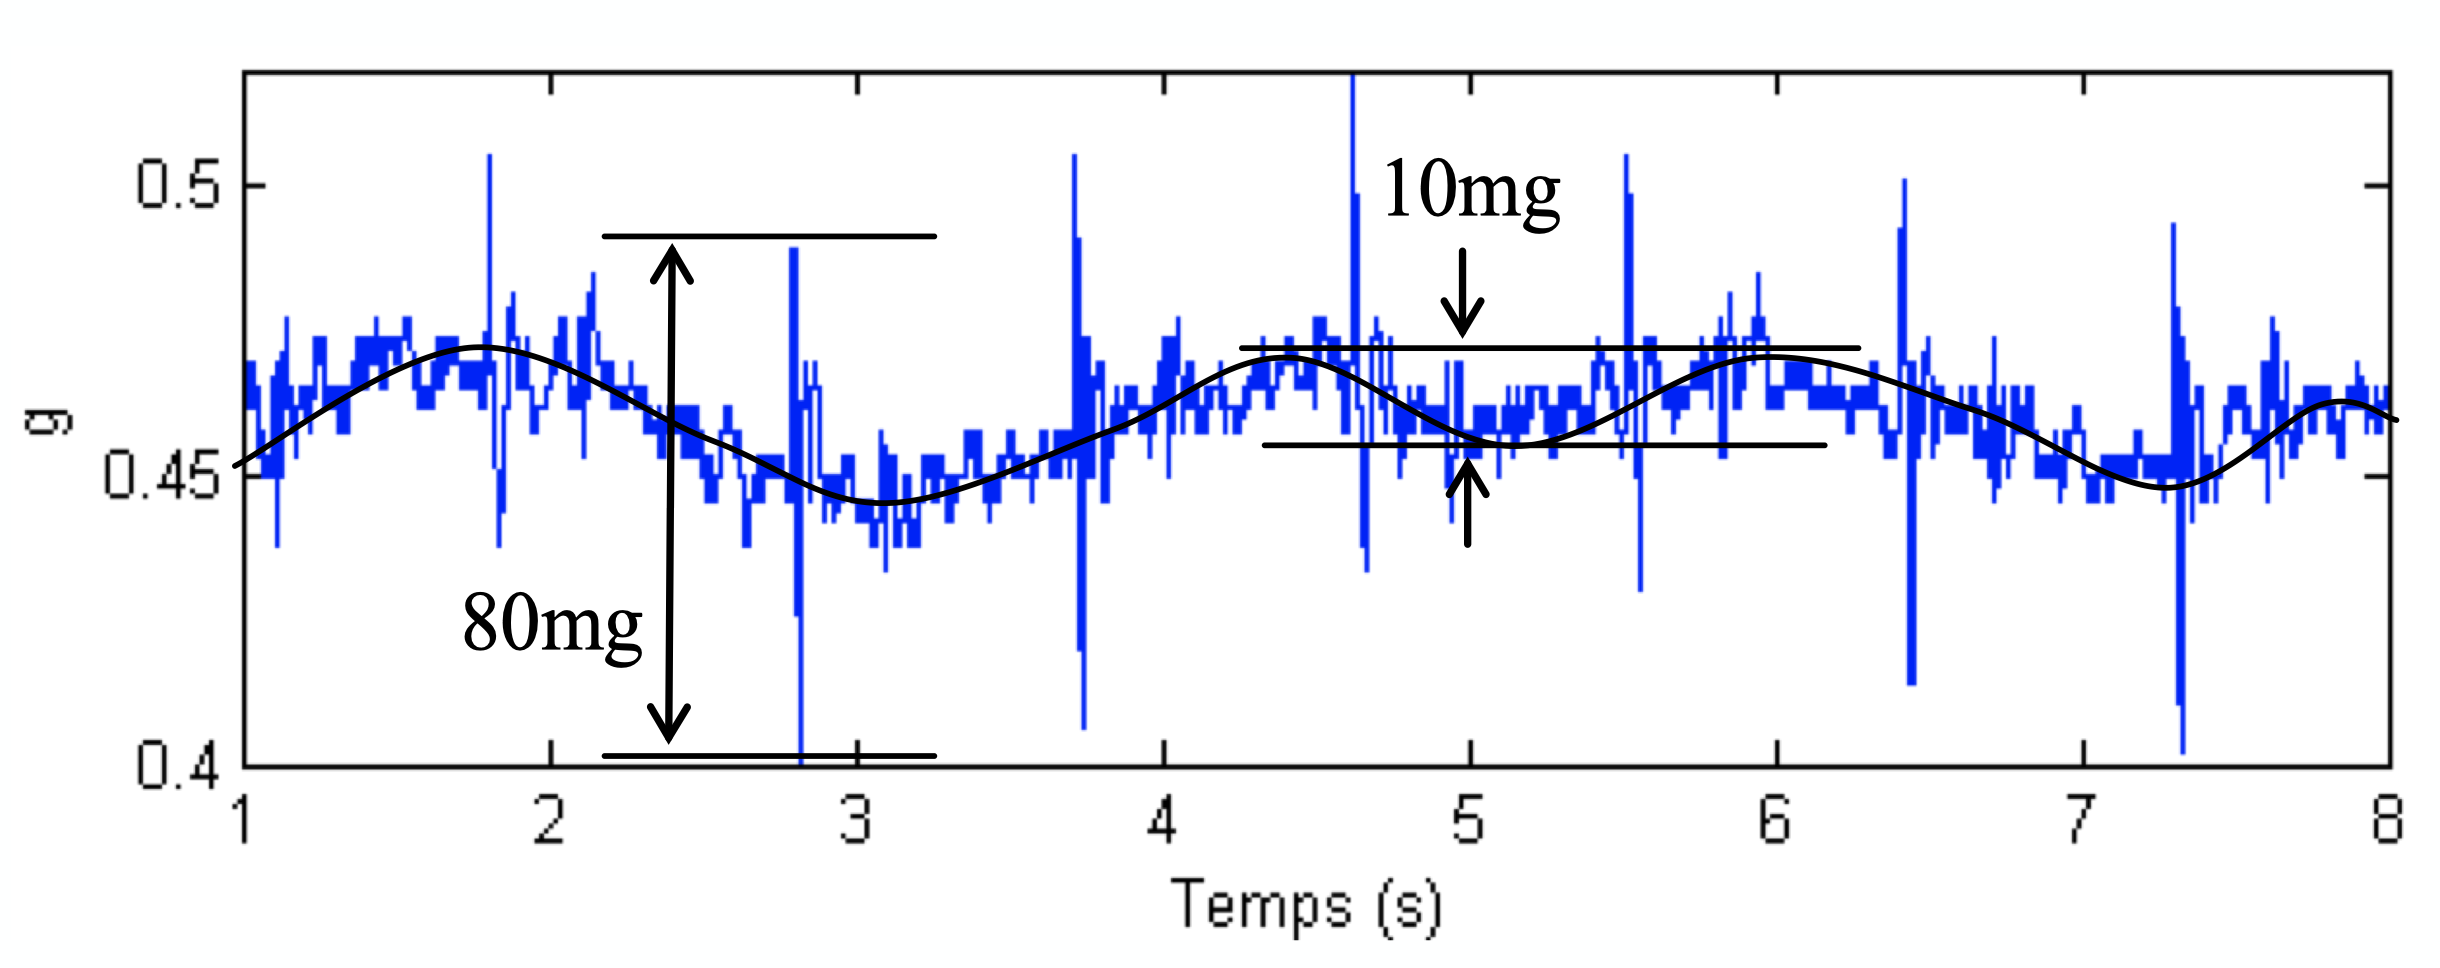
\includegraphics[width=1\textwidth]{imu_research/Paper_Hung_rawData}
    \caption{Rohdaten des Accelerometers in \cite{hung_central_2018}}
    \label{imu_research_hung_rawData}
\end{figure}

Hierbei wurde ein Bandpassfilter mit adaptiver Anpassung verwendet, um den SNR (\textit{signal-noise-ratio}) zu optimieren.
Der Puls wurde ermittelt, indem Peaks (Max: \textit{V}-Peak, Min: \textit{R}-Peak) gefunden und als Herzschlag interpretiert wurden.
Bei der Atmung musste Signalrauschen, z.B von der Reibung des T-Shirts und Haut, herausgefiltert werden. 
Es wurden 3 Features anhand der Amplitude über die Zeit berechnet. 
\begin{itemize}
    \item Spectral ratio
    \item Wavelet coefficients
    \item Linear prediction coefficients
\end{itemize}
\todo{Dieses itemize beschreiben und auf deutsch}

Zudem wurden nichtlineare Features in betracht gezogen.
\begin{itemize}
    \item Poincare plot geometry
    \item Detrended Fluctuation Analysis
    \item Approximate Entropy
    \item Largest Lyapunov exponent
\end{itemize}
\todo{Dieses itemize beschreiben und auf deutsch}

Die Features wurden anschließend mit der \textit{ANOVA-Toolbox} ausgewertet.
Somit konnte ermittelt werden, ob in dem zeitlichen Intervall ein Apnoe vorgekommen ist, oder nicht.

Durch dieses Paper wurde eine Genauigkeit von 84.2\% erreicht, ein zentrales Apnoe zu erkennen und mit 84.1\% konnte ermittelt werden, dass in diesem Zeitrahmen kein zentrales Apnoe vorkam.


\subsection{Google Glass Brille zur Detektion direkt am Kopf}
\todo{optimize title}
2015 wurde erforscht, durch Informationen des Google Glass Puls und Atemsignal zu ermitteln \cite{hernandez_cardiac_nodate}. 
Der Vorteil hierbei ist die Position der Brille. 
Da sie Am Kopf platziert ist, liefert die Brille möglicherweise vielversprechende Werte, im Vergleich zu IMU-Daten, die am Brustkorb aufgezeichnet worden sind.
Das Google Glass wurde nicht entwickelt, um physiologische Daten zu sammeln, kann jedoch dafür verwendet werden, da alle nötigen Sensoren (Accelerometer, Gyroscope und Kamera) vorhanden sind.
\todo{write about the 2 sections: Pulse wave, respiratory wave}
\todo{write, how the results were}

\begin{figure}[ht]
    \centering
    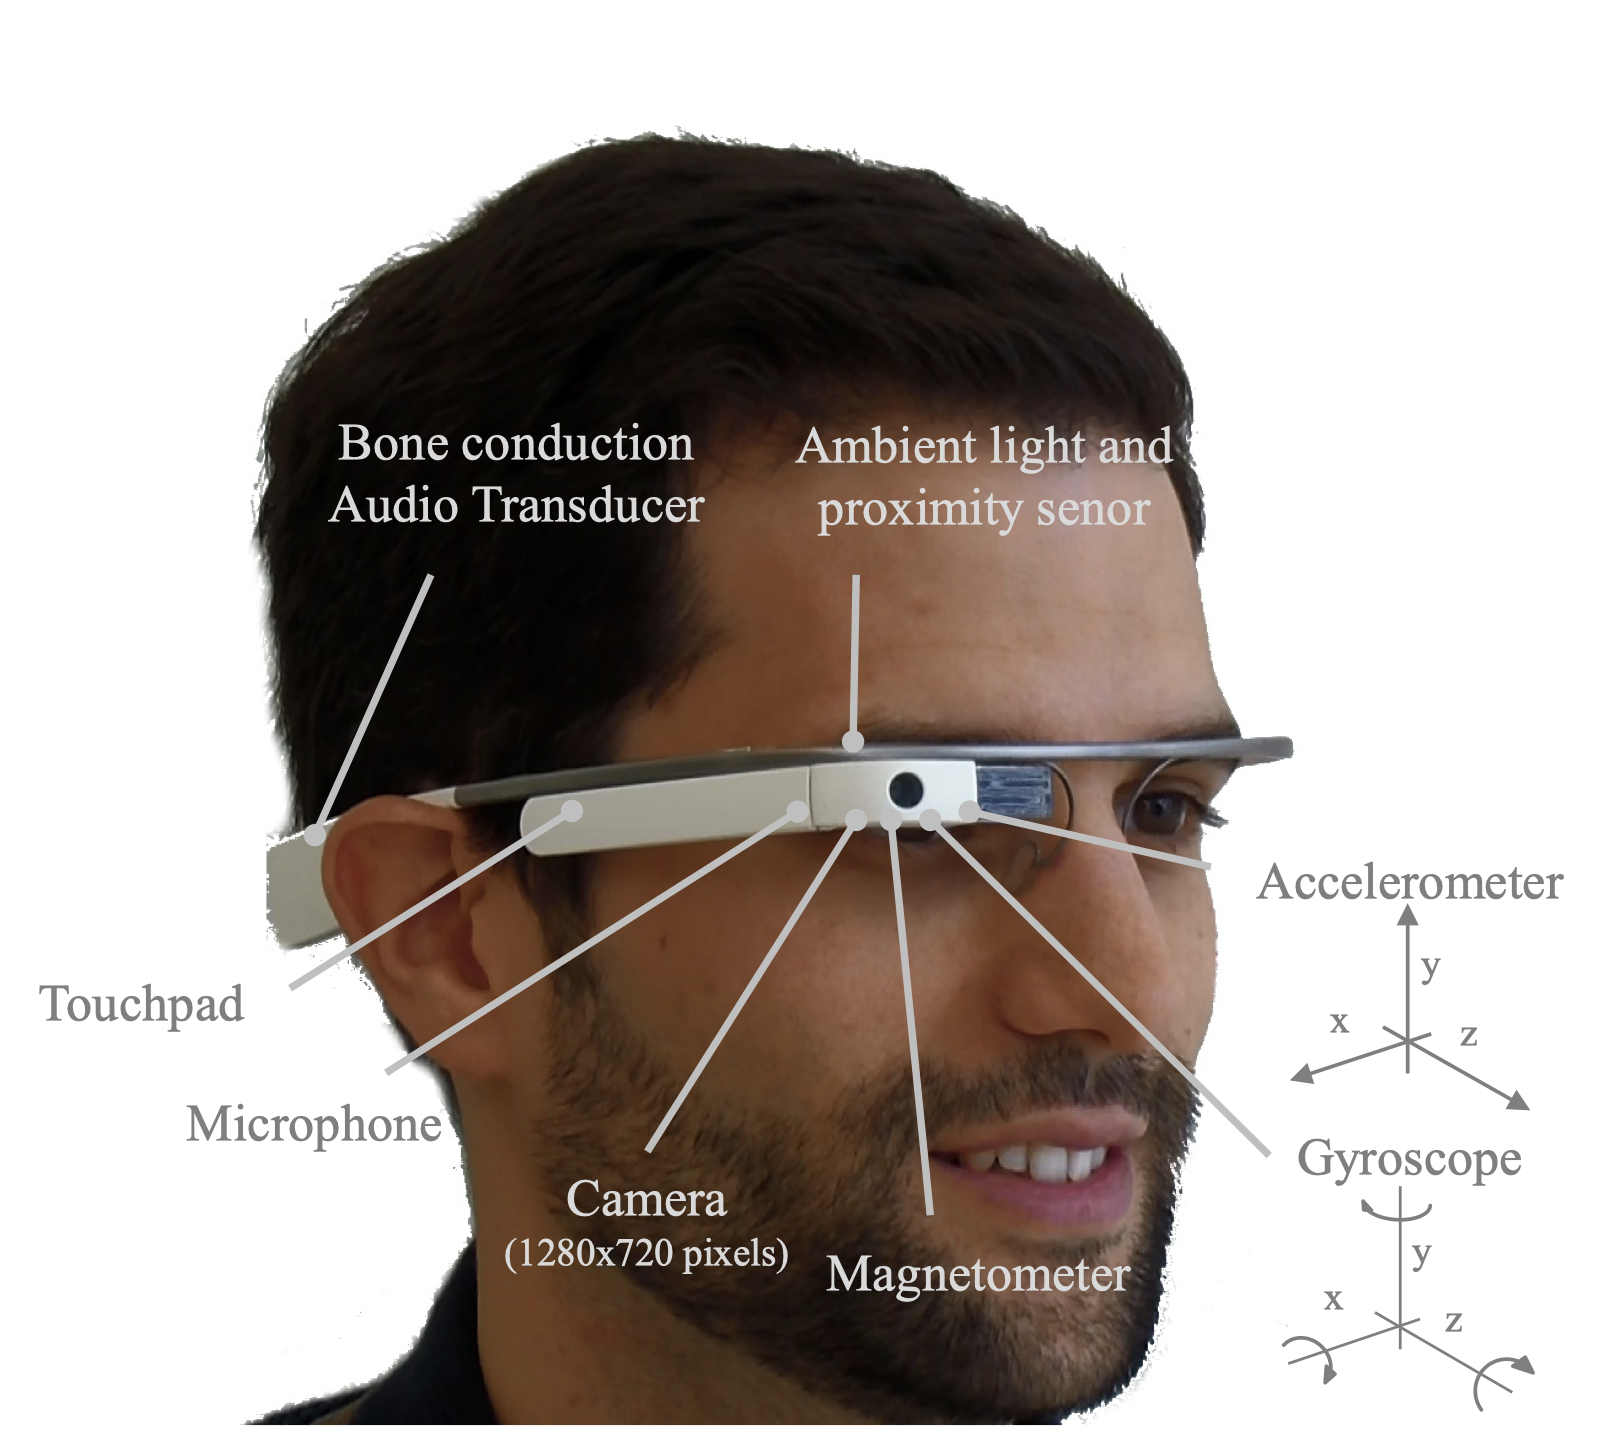
\includegraphics[width=\textwidth / 2]{imu_research/googleGlass}
    \caption{Google Glass Sensordaten \cite{hernandez_cardiac_nodate}}
    \label{imu_research_google_glass}
\end{figure}

\subsection{Überwachung von Puls und Atmung mittels eSense-Earpods}
2019 wurde von \textit{Tobias Röddiger}, \textit{Daniel Wolffram} und \textit{David Laubenstein} nachgewiesen, dass es möglich ist, mittels den eSense-Earpods die Atmung und den Puls näherungsweise zu ermitteln \cite{roddiger_towards_2019}. 
Dies gelang etwas genauer, als das Monitoring von \textit{J. Hernandez} mit dem Google Glass \cite{hernandez_cardiac_nodate}
Es wurden hierbei eine Studie mit 12 Personen aufgezeichnet, welche in 3 Positionen (liegend, stehend, sitzend) jeweils vor, bzw. nach einer sportlichen Bewegungsphase einen einminütigen Atemablauf durchgeführt haben. 
Die Analyse der Daten erfolgte im Anschluss der Studie und wurde in einer Pipeline verarbeitet, welche zuerst das Rauschen reduziert, anschließend einen Triangle-Filter der Breite $2\si{\s}$ anwendet und danach eine PCA (engl. \textit{principal component analysis}) ausführt, um die Daten unabhängig von deren Achse zu bewerten.
Nun wurden Windows mit der Größe von $20\si{\s}$ extrahiert, welche die die Atmung und den Puls anhand dieses Windows berechnen.
Die Resultate ergaben einen mittleren absoluten Fehler (engl. \textit{mean absolute error}) von 2.62 CPM (acc) und 2.55 CPM (gyro), jedoch variieren diese von Proband zu Proband.